\documentclass[12pt,oneside,a4paper,parskip]{scrbook}
\usepackage[utf8]{inputenc}
\usepackage{csquotes}
\usepackage[english]{babel}
\usepackage{floatflt} 
\usepackage{subfigure}
\usepackage[pdftex]{graphicx}
\usepackage[hidelinks]{hyperref}
\usepackage{color}
\usepackage{amssymb}
\usepackage{amsmath}
\usepackage{textcomp}
\usepackage{nicefrac}
\usepackage{pdfpages}
\usepackage{float} 
\usepackage{pdflscape}
\usepackage{subfigure}
\usepackage{pdfpages}  
\usepackage[verbose]{placeins} 
\usepackage[nouppercase,headsepline,plainfootsepline]{scrpage2}
\usepackage{listings}		
\usepackage{xcolor}			
\usepackage{color}			
\usepackage{caption}		
\usepackage{subfigure}			
\usepackage{epstopdf}		
\usepackage{longtable}  
\usepackage{setspace}
\usepackage{booktabs}
\usepackage[style=numeric]{biblatex}
\addbibresource{bib_file.bib}
\bibliography{bib_file}
\graphicspath{ {C:/informatik/7.Semester/BachlorArbeit/figures/} }


%%%%%%%%%%%%%%%%%%%
%% definitions
%%%%%%%%%%%%%%%%%%%
\def\BaAuthor{Florian Hohn}
\def\BaTitle{Evaluation and implementation of gradient descent algorithms on streaming data}
\def\BaSupervisorOne{Prof.\ Dr.\ Frank-Michael Schleif}
\def\BaSupervisorTwo{Moritz Heusinger}
\def\BaDeadline{25.02.2020}

\hypersetup{
pdfauthor={\BaAuthor},
pdftitle={\BaTitle},
pdfsubject={Subject},
pdfkeywords={Keywords}
}

\newcommand{\R}{\mathbb{R}}

%%%%%%%%%%%%%%%%%%%
%% configs to include
%%%%%%%%%%%%%%%%%%%
\colorlet{punct}{red!60!black}
\definecolor{background}{HTML}{EEEEEE}
\definecolor{delim}{RGB}{20,105,176}
\colorlet{numb}{magenta!60!black}

\definecolor{gray}{rgb}{0.4,0.4,0.4}
\definecolor{darkblue}{rgb}{0.0,0.0,0.6}
\definecolor{cyan}{rgb}{0.0,0.6,0.6}

\definecolor{pblue}{rgb}{0.13,0.13,1}
\definecolor{pgreen}{rgb}{0,0.5,0}
\definecolor{pred}{rgb}{0.9,0,0}
\definecolor{pgrey}{rgb}{0.46,0.45,0.48}

\lstset{
  basicstyle=\ttfamily,
  columns=fullflexible,
  showstringspaces=false,
  commentstyle=\color{gray}\upshape
  linewidth=\textwidth
}

\lstdefinelanguage{json}{
    basicstyle=\normalfont\ttfamily,
    numbers=left,
    numberstyle=\scriptsize,
    stepnumber=1,
    numbersep=8pt,
    showstringspaces=false,
    breaklines=true,
    backgroundcolor=\color{background},
    literate=
     *{0}{{{\color{numb}0}}}{1}
      {1}{{{\color{numb}1}}}{1}
      {2}{{{\color{numb}2}}}{1}
      {3}{{{\color{numb}3}}}{1}
      {4}{{{\color{numb}4}}}{1}
      {5}{{{\color{numb}5}}}{1}
      {6}{{{\color{numb}6}}}{1}
      {7}{{{\color{numb}7}}}{1}
      {8}{{{\color{numb}8}}}{1}
      {9}{{{\color{numb}9}}}{1}
      {:}{{{\color{punct}{:}}}}{1}
      {,}{{{\color{punct}{,}}}}{1}
      {\{}{{{\color{delim}{\{}}}}{1}
      {\}}{{{\color{delim}{\}}}}}{1}
      {[}{{{\color{delim}{[}}}}{1}
      {]}{{{\color{delim}{]}}}}{1},
}

\lstset{language=xml,
  morestring=[b]",
  morestring=[s]{>}{<},
  morecomment=[s]{<?}{?>},
  stringstyle=\color{black},
  numbers=left,
  numberstyle=\scriptsize,
  stepnumber=1,
  numbersep=8pt,
  identifierstyle=\color{darkblue},
  keywordstyle=\color{cyan},
  backgroundcolor=\color{background},
  morekeywords={xmlns,version,type}% list your attributes here
}

\lstset{language=Java,
  showspaces=false,
  showtabs=false,
  tabsize=4,
  breaklines=true,
  keepspaces=true,      
  numbers=left,
  numberstyle=\scriptsize,
  stepnumber=1,
  numbersep=8pt,
  showstringspaces=false,
  breakatwhitespace=true,
  commentstyle=\color{pgreen},
  keywordstyle=\color{pblue},
  stringstyle=\color{pred},
  basicstyle=\ttfamily,
  backgroundcolor=\color{background},
%  moredelim=[il][\textcolor{pgrey}]{$$},
%  moredelim=[is][\textcolor{pgrey}]{\%\%}{\%\%}
}




\begin{document}


%%%%%%%%%%%%%%%%%%%
%% Titelseite
%%%%%%%%%%%%%%%%%%%


\frontmatter
\titlehead{%  {\centering Seitenkopf}
  {University of Applied Sciences W\"{u}rzburg-Schweinfurt
  Faculty of Computer Science and Business Information Systems}}
\subject{Bachelor-Thesis}
\title{\BaTitle\\[15mm]}
\subtitle{\normalsize{submitted to the University of Applied Sciences W\"{u}rzburg-Schweinfurt in the Faculty of Computer Science and Business Information Systems to achieve the Bachelor of Engineering degree in 'Information Systems'}}
\author{\BaAuthor}
\date{\normalsize{Submitted on: \BaDeadline}}
\publishers{
  \normalsize{First Reader: \BaSupervisorOne}\\
  \normalsize{Second Reader: \BaSupervisorTwo}\\
}

%\uppertitleback{ }
%\lowertitleback{ }

\maketitle


%%%%%%%%%%%%%%%%%%%
%% abstract
%%%%%%%%%%%%%%%%%%%

\section*{Summary}

TODO

\section*{Abstract}

TODO

\newpage
\chapter*{Note of thanks}



%%%%%%%%%%%%%%%%%%%
%% Table of Contents
%%%%%%%%%%%%%%%%%%%
\tableofcontents	




%%%%%%%%%%%%%%%%%%%
%% Main part of the thesis
%%%%%%%%%%%%%%%%%%%
\mainmatter

\chapter{Introduction}\label{ch:intro}

\chapter{Basics}
The Goal of this Chapter is to give the Reader a basic understanding of how Machine Learning Algorithm work. 
Furthermore, it will describe what the difference is between unsupervised und supervised learning. 

There will be also an introduction and description on how the Gradient Descent Algorithm, that is the basis for the 
Modified versions of the Algorithms that will be compared in this work, works and how it decides what to do. 
After this is done there will be also a short description on what Streaming Data is and on the framework that is used to 
realise the implementation of the Experiments.

Finally there will be a explanation on how the criteria for the comparission of the Algorithms where choosen and how 
theses criteria work.

\section{Machine Learning}

The term 'Machine Learning' stands for a collection of self-learning algorithms, that learn form input Data to make 
fast and correct decisions and predictions. It is importand to remember that it is not a real Artifical inteligence, 
but rather a sequence of statistical analyses on given data, with the goal to make gradualy improvments to the prediction 
models of the algorithm.  
A Machine can do this optimization alot faster and effectifly than a humans, especially if this optimization has to be 
done in real time on big data input sets. This give also a bigger flexability, as machine that can learn from a changing 
enviroment needs lesser redesigns, which leads to less time that gets wastet and can be used more productifly on other 
tasks. 

All these are reasons why Machine Learning has an ever increasing importants in the field of computer science, 
but also an growing impact on everday life. It is thanks to Machine learning that there are intelligent assisstant 
softwares that can recognize voice commands and questions (Apples SIRI, Amazon Alexa or Microsofts Cortana),
e-mail spam filter, nearly self-driving cars, reliable search-engines, faster and more precise weather forecasts and 
challenging game ai's nowadays 

Machine Learning Algorithms can be categorisized depending on how they learn from the available training Data to create 
a model for the predictions. There are three main subdivisions, under wich these algorithms can fall. 
The first one is the Supervised learning strategy, then the Unsupervised learning strategy and the Reinforced learning 
strategy. 

\begin{figure}
  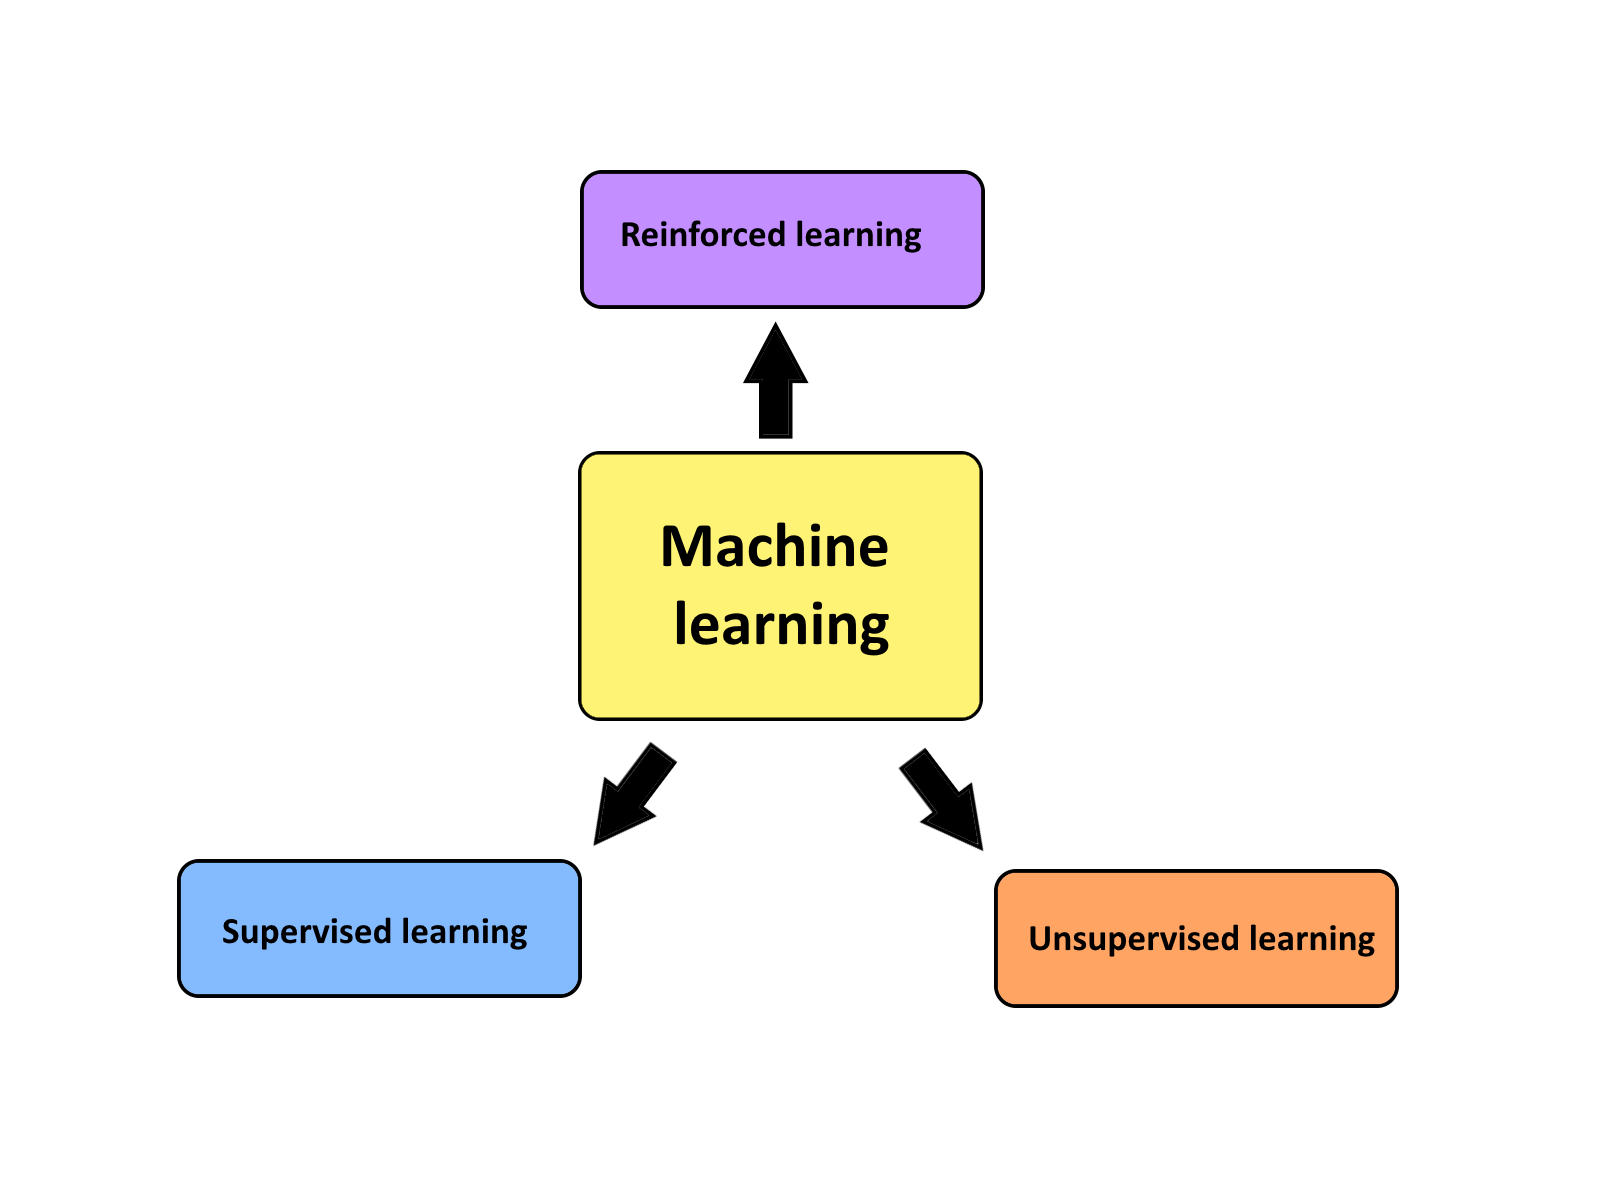
\includegraphics[width=\linewidth]{Overview_ml}
  \caption{Overview of the Machine Learning Strategy's.}
  \label{fig:overview_ML}
\end{figure}

Only the Supervised Learning strategy will be explained in more detail on the following pages, as the focus of this 
thesis lays in the comparission of several different implementations of classification algortihms that are based on 
Supervised Learning.
 

\cite{IntroML}

\subsection{Supervised Learning}

The idea behind Supervised learning is to create a model from a already labeled training data set, that then can make 
prediction and decision on new or unknown data based on the learned model from the training set. 
The following example will help to understand this easier.
Lets say a fruit farmer wants to automatically sort the harvested Fruits in either categorie A or B for the market. 
The sorting device is equiepped with 2 sensors to measure 2 features, one for colour and another one for the size of the 
fruit. It then decides to wich of the two classes the fruit belongs to. As this is a System that is capable of dividing 
features into a discrete number of classes the system can be called a \textit{classifier}. 
This is a typical exampel of an \textit{classifiecation task}.
To configure the System in such a way that it correctly sorts the fruits into the right category, 
a specailist hand picks several fruits from a small test set and then sorts them depending on the already named features. 
In other words, the specailist classiefies them. Based on this by hand sortet training set the machine will then later 
decide how the other fruits should be sorted. It is used as a \textit{model} for the classification. \cite{IntroAI}
Another type of Supervised learning is the \textit{regression task}. The difference to the \textit{classification task} is, 
that instead of a \textit{discrete} number of classes that gets returned, a \textit{continous} number of classes will be 
returned. An example of a \textit{regressive task} is, for example, the prediction of the Stock market or the price of 
medications.

The Process as seen in figure \ref{fig:sl_process} and as described as in the example of the farmer and his sorted 
fruits shows how the supervised learning works. The Algorithm (marked in green) learns with the help of the labeled 
training data. The result of this learning is then that the trained Algorithm, now called predictive model, 
can be used in a production enviroment.
New, unlabeled, data can then be send into the predictiv model to get a predictied model as an output. \cite{PythonML}

To better understand how this predictiv model is formed, one has to understand how the classification task works. 
In the classification task the computer programm is asked to specify which of \textit{k} catergories a input belongs to. 
To solve this task, the learning algorithm is usually asked to produce a function \textit{f} : $\R{}$ $\rightarrow$ ${1,...,k}$. 
When \textit{y} = \textit{f}(\textit{\textbf{x}}), the model assigns an input described by vector \textit{\textbf{x}} to a 
category identified by numeric code \textit{y}.
There are other variants of the classification task, for example, where \textit{f} outputs a probability distribution over 
classes. An example of a classification task is object recognition, where the input is an image (usually described as a set 
of pixel brightness values), and the output is a numeric code identifying the object in the image. \cite{Goodfellow-et-al-2016}

\pagebreak

\begin{figure}
  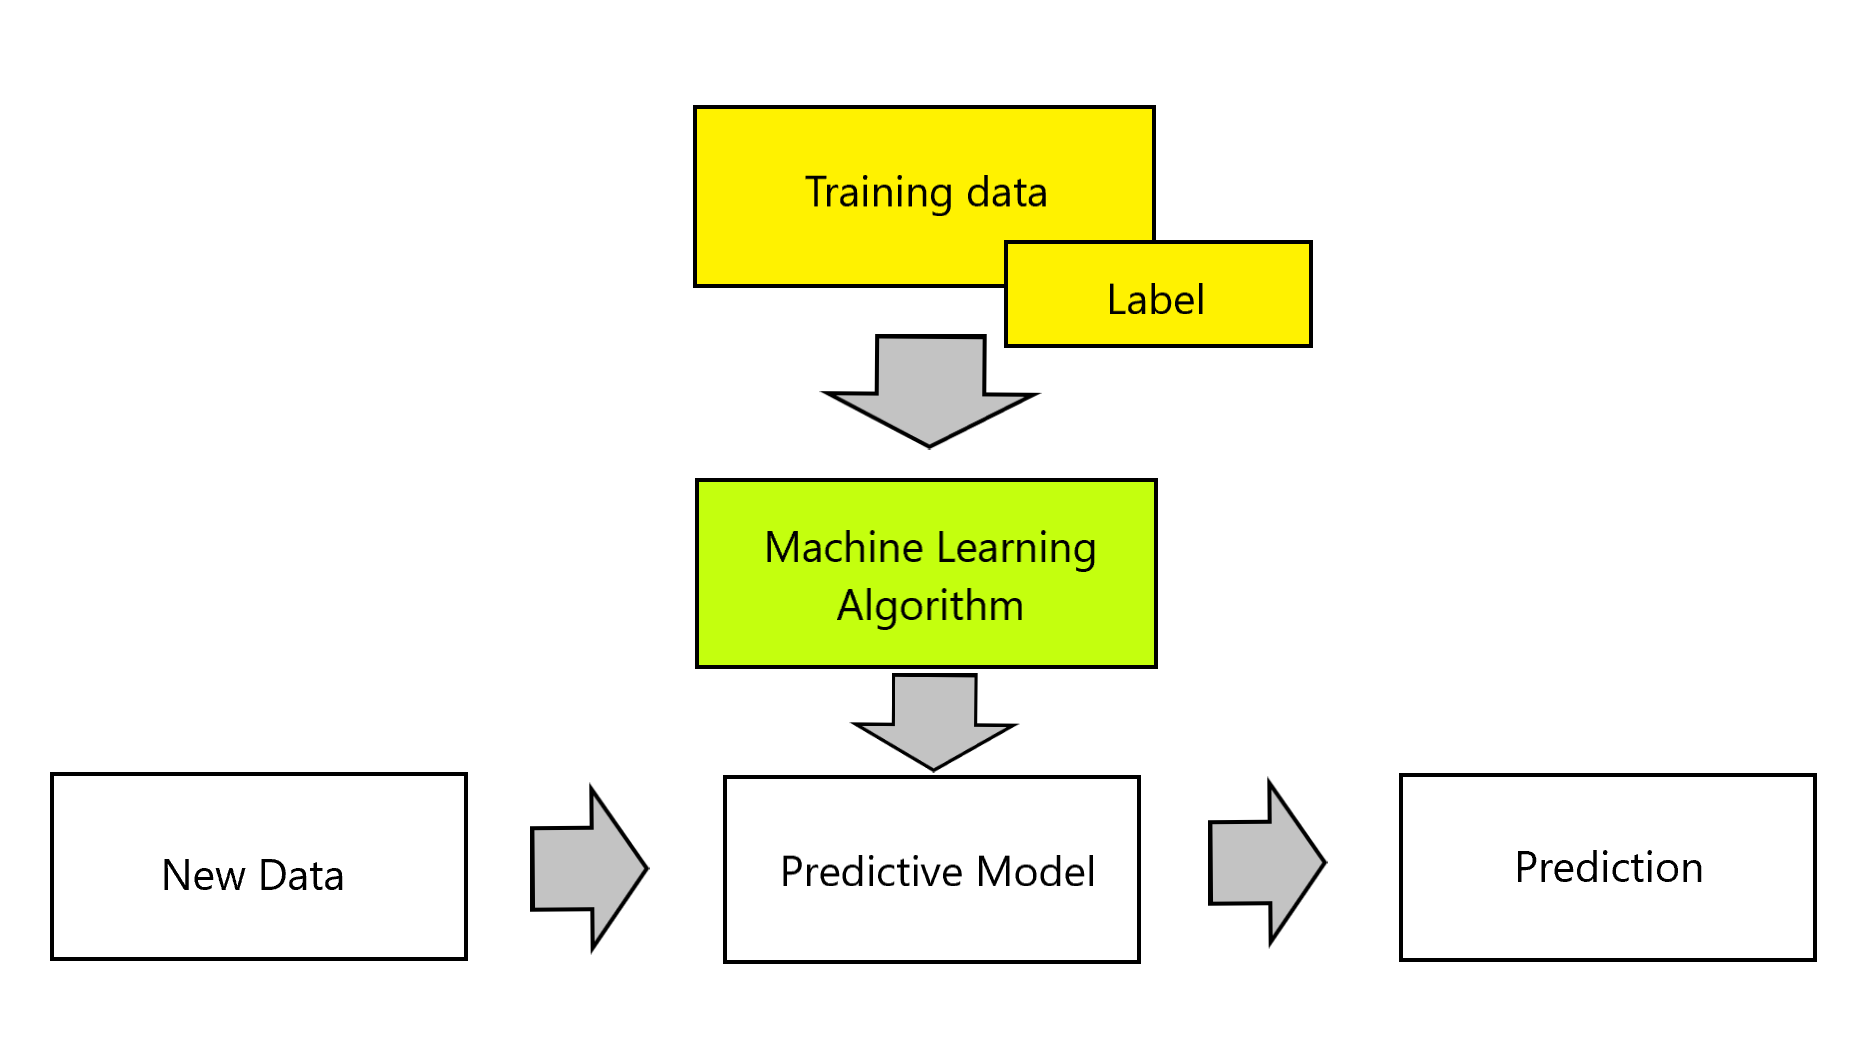
\includegraphics[width=\linewidth]{SL_process_figure}
  \caption{Process of the Supervised Learning. \cite{PythonML}}
  \label{fig:sl_process}
\end{figure}

Then there must be also differentiated between the type of data that is put into the classification process.
In batch or offine classification, a classifier-building algorithm is given a set of labeled examples. 
The algorithm creates a model, a classifier in this case. The model is then deployed, that is, used to predict the label 
for unlabeled instances that the classifier builder never saw. If we go into more detail, we know that it is good 
methodology in the first phase to split the dataset available into two parts, the training and the testing dataset, 
or to resort to cross-validation, to make sure that the classifier is reasonably accurate.
But in any case, there is a first training phase, clearly separated in time from the prediction phase.

In the online setting, and in particular in streaming, like it is this thesis, this separation between training, 
evaluating, and testing is far less clear-cut, and is interleaved. We need to start making predictions before we have all 
the data, because the data may never end. We need to use the data whose label we predict to keep training the model, 
if possible. And probably we need to continuously evaluate the model in some way to decide if the model needs more or 
less aggressive retraining. \cite{MLonDataStreams}

\pagebreak

\subsection{Gradient Descent}
The Gradient descent Algorithm is one of the most popular Algorithms to perform optimizations on and is by far the most 
commen way to optimize neural networks.This is also the reason why nearly every state-of-the-art Deep learning library 
has various forms of implementations to perform optimization on the gradient descent. The Problem, however is, that these
Algorithms often perform as some form of black-box, because a practical explanation of what their stengths and weaknesses 
is are hard to find and explain.
Gradient descent is a way to minimize an objective function \textit{J}($\theta$) parameterizedby a model's parameters $\theta \in \R{}^d$ by 
updating the parameters in the opposite directionof the gradient of the objective function $\nabla_\theta \in $\textit{J}($\theta$) with respect to 
the parameters. The learning rate $\eta$ determines the size of the steps wetake to reach a local minimum. In other words, 
we follow the direction of the slopeof the surface created by the objective function downhill until we reach a valley. \cite{overvieDiffRSLVQ}

The normal gradient descent, also known as batch-gradient descent, computes the gradient of the functionwith 
respect to the parameters $\theta$ for the entire training set:

\begin{equation}
\theta = \theta - \eta * \nabla_\theta \textit{J}(\theta)
\end{equation}

Since we need to calculate the gradients for the complete dataset to get just one update, batch gradient descent can get very
slow and is intractable for dataset that do not fit into the memory. For this reason the batch gradient descent implementation can not be used in this comparison,
as it is not able to perform updates "on-the-fly", as this is a necessarity for use on streaming Data. 

In contrast to that, the Stocastic Gradient Descent (short: SGD) can perform a update for \textit{each} training example
$\textit{x}^\textit{(i)}$ and label $\textit{y}^\textit{(i)}$:

\begin{equation}
\theta = \theta - \eta * \nabla_\theta \textit{J}(\theta;\textit{x}^\textit{(i)};\textit{y}^\textit{(i)})
\end{equation}

While the bacht gradient descent performed redudant computations for large datasets, as it recomputes gradients for similar examples 
before each update, the SGD puts away this redundacy by performing one update at a time. Because of that it performce much faster and 
can be used on Streaming Data.
The SGD performs frequent updates with a high variance, that causes the objective function to fluctuate heavily. 

\begin{figure}
  \centering
  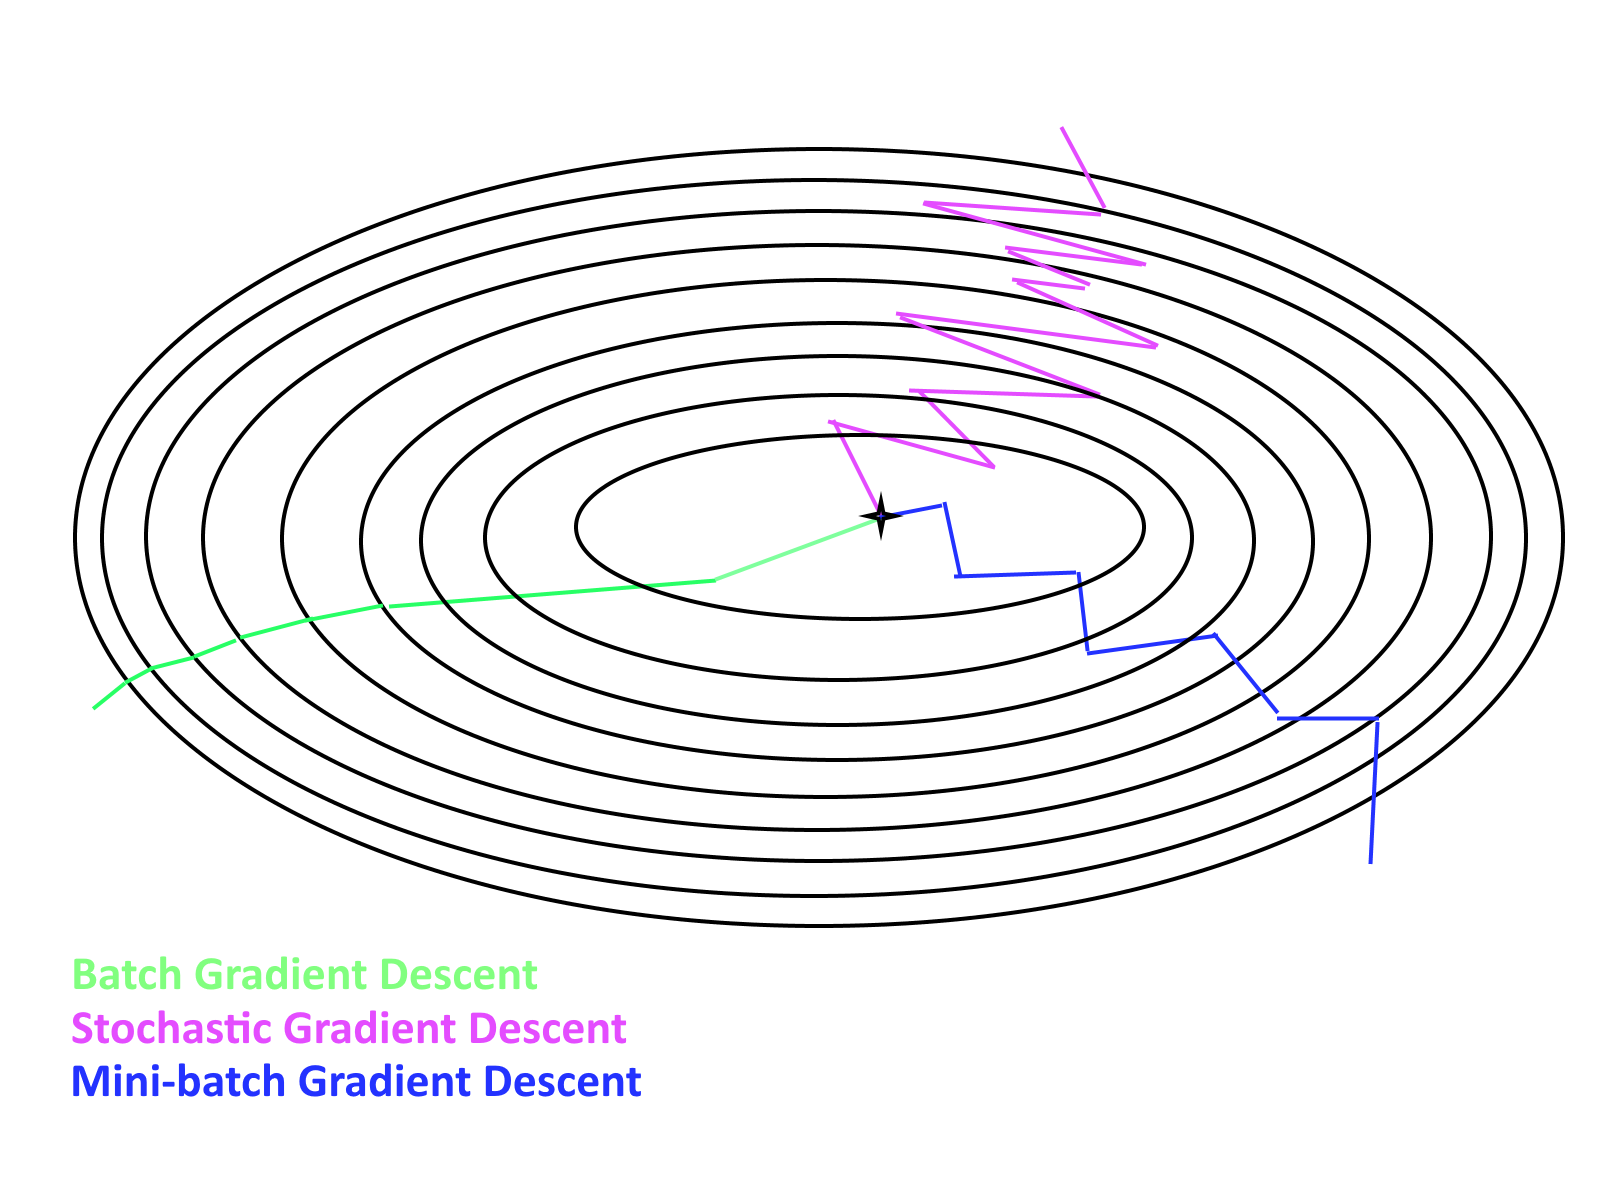
\includegraphics[width=0.7\columnwidth]{Gradient_desc_types}
  \caption{Visualisation differences of the three Gradient Descent Algorithms}
  \label{fig:comp_GD}
\end{figure}

This fluctuation enables the SGD to jump to new and potetially better local minima, while the batch gradient only converges 
to the minimum of the basin the parameters are placed in. But this also ultimatly complicates the convergensto the exact minimum, 
as the SGD keeps overshooting. This can be fixed by slowly decreasing the learning rate, as the SGD then shows the same 
convergeance behaviour as the batch gradient descent. It then almost certainly converges to a local or gloabl minimum for
non-convex and convex optimization respectivly. \cite{overvieDiffRSLVQ}
These advantages lead to the fact that the SGD is the most common Gradient descent algorithm.

Then there is also the Mini-batch gradient descent algorithm. It takes the best of both worlds and performs an update for
every mini-batch on \textit{n} training examples:

\begin{equation}
\theta = \theta - \eta * \nabla_\theta \textit{J}(\theta;\textit{x}^\textit{(i:i+n)};\textit{y}^\textit{(i:i+n)})
\end{equation}

This way it reduces the variance of the parameter updates, which can lead to a more stable convergence.
It can also make use of highly optimized matrix optimizations common for state-of-the-art deep learning libraries,
that makes computing the gradient with respect to a mini-batch very efficient. 
Common mini-batch sizes range between 50 and 256 , but can vary for different applications. Typically the Mini-batch gradient descent is the 
algorithm of choice when there is a neural network to train and the term SGD is usually also employed even when a mini-batches
are used. \cite{overvieDiffRSLVQ}

\pagebreak

\section{Streaming Data}

Data streams are an algorithmic abstraction to support real-time analytics. They are sequences of items, 
possibly infinite, each item having a timestamp, and so a temporal order. Data items arrive one by one, 
and we would like to build and maintain models, such as patterns or predictors, of these items in real time. 
There are two main algorithmic challenges when dealing with streaming data: the stream is large and fast, 
and we need to extract information in real time from it. That means that usually we need to accept approximate 
solutions in order to use less time and memory.
Also, the data may be evolving, so our models have to adapt when there are changes in the data. \cite{MLonDataStreams}

\subsection{Challenges with Streaming Data}

\section{Framework}

\subsection{SCIKIT Multiflow}

\section{Criteria for the Comparission}

\subsection{Performance}

\subsection{Accuracy}

\subsection{*kappa-errors}

\chapter{Used Algorithms}

\section{Theoretical Work}
This chapter will try to give a short explanation about how the Robust Soft Learning Vector Quantization Algorithm 
(short: RSLVQ) works and will also explain the algorithm that it is based on. 
Furthermore will it explain what momentum based gradient descent algortihms there are and how they work.
These are used in the different optimization implementation of the RSLVQ that will be compared in the later chapters. 

\section{Learning Vector Quantization}

\section{Robust Soft Learning Vector Quantization}

\section{Momentum Based Gradient Descent}
The following section will outline three algorithms that are widely used in the Deep learning Community and that will later
be used to optimize the RSLVQ Algorithm in hopes to improve its performence and accuracy.

\subsection{Momentum}
SGD has trouble navigating ravines, i.e. areas where the surface curves much more steeply in one dimension than in another \cite{problemSteepLearn, Ruder2016AnOO},
which are common around local optima. In these scenarios, SGD oscillates across the slopes of the ravine while only making 
hesitant progress along the bottom towards the local optimum as in figure.

\begin{figure}
  \centering
  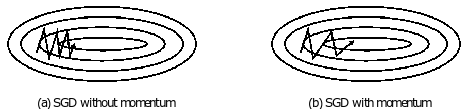
\includegraphics[width=\columnwidth]{SGD_momentum}
  \caption[Diff. SGD moment.]{Differences of a SGD with and without momentum.\footnotemark} 
  \label{fig:SGD_momentum}
\end{figure}

Momentum \cite{QIAN1999145, Ruder2016AnOO} is a method that helps accelerate SGD in the relevant direction and dampens
oscillations as can be seen in figure . It does this by adding a fraction $\gamma $ of the update vector of the past time step to the
current update vector

\begin{equation}
\begin{split}
\textit{v}_\textit{t} = \gamma\textit{v}_\textit{t-1} + \eta \theta - \eta\nabla_\theta \textit{J}(\theta) \\
\theta = \theta - \textit{v}_\textit{t}
\end{split}
\end{equation}

The momentum term $\gamma $ is usualy set to 0.9 or a similar value.

In his Article, Ruder \cite{overvieDiffRSLVQ} describs it like if we would push a ball down a hill. 
The ball accumulates momentum as long as it rolls downhill, becoming faster and faster on the way 
(until it reaches its terminal velocity, if there is air resistance, i.e. $\gamma $ < 1). 
The same thing happens to our parameter updates: The momentum term increases for dimensions whose gradients
point in the same directions and reduces updates for dimensions whose gradients change directions.
As a result, we gain faster convergence and reduced oscillation.
\footnotetext{Genevieve B. Orr}

\subsection{Adadelta}
One of the more often used momentum-based Algorithm is the Adadelta approach. It is an extension of the Adagrad \cite{Zeiler2012ADADELTAAA} that 
seeks to reduce its aggressive, monotonically decreasing learning rate. Instead of accumulating all past squared gradients, 
Adadelta restricts the window of accumulated past gradients to some fixed size $\omega$.  

Rather than inefficently storeing $\omega$ previous squared gradients, the sum of gradients is recursively defined as a 
decaying average of all past squared gradients. The running average $\textit{E}[\textit{g}^2]_t$  at time step \textit{t} 
then depends (as a fraction $\gamma $ similarly to the Momentum term) only on the previous average and the 
current gradient:

\begin{equation}
\textit{E}[\textit{g}^2]_t = \gamma\textit{E}[\textit{g}^2]_t-1 + (1-\gamma)\textit{g}^2_t
\end{equation}

We then set $\gamma$ to a simliar value as the momentum, around 0.9. The SGD update will then be rewriten in terms of the 
parameter update vector $\Delta\theta_\textit{t}$:

\begin{equation}
  \begin{split}
    \Delta\theta_\textit{t} = -\eta \cdot \textit{g}_\textit{t,i} \\
    \theta_\textit{t+1} = \theta_\textit{t} - \Delta\theta_\textit{t}
  \end{split}
\end{equation}

Bacuase of this, the parameter update vector, that is base of the parameter update vecot of the Adagrad, takes the form of:

\begin{equation}
  \Delta\theta_\textit{t} = -\frac{\eta}{\sqrt{\textit{G}_\textit{t} + \epsilon}} \odot \textit{g}_\textit{t}
\end{equation}

In the next step the diagnoal Matrix $\textit{G}_t$ gets replaced with the decaying average over past squared gradients 
$\textit{E}[\textit{g}^2]_\textit{t}$:

\begin{equation}
  \Delta\theta_\textit{t} = -\frac{\eta}{\sqrt{\textit{E}[\textit{g}^2]_\textit{t} + \epsilon}} \textit{g}_\textit{t}
\end{equation}

As the denominator is just the root mean squared (RMS) error criterion of the gradient, we can replace
it with the criterion short-hand: 

\begin{equation}
  \Delta\theta_\textit{t} = -\frac{\eta}{RMS[\textit{g}]_t} \textit{g}_\textit{t}
\end{equation}

As in \cite{AdadeltaAddition} noted, the units in this update (as well as in the SGD, Momentum and Adagrad) do not match,
i.e. the update should have the same hypothetical units as the parameter. To realize this, they first define another 
ecaying average, this time not of squared gradients but of squared parameter updates:

\begin{equation}
  \textit{E}[\Delta\theta^2]_t = \gamma\textit{E}[\Delta\theta^2]_t-1 + (1-\gamma)\Delta\theta^2_t
\end{equation}

This leads to that the root mean squared error of the parameter updates is:

\begin{equation}
  \textit{RMS}[\Delta\theta]_t = \sqrt{\textit{E}[\Delta\theta^2]_t + \epsilon}
\end{equation}

Because the $\textit{RMS}[\Delta\theta]_t$ value is unknown to us, we try to approximate it with the \textit{RMS} of 
parameter updates until the previous time step. Replacing the learning rate $\eta$ in the previous update rule with $\textit{RMS}[\nabla\theta]_t-1$
leads to the final update rule for the Adadelta:

\begin{equation}
  \begin{split}
  \Delta\theta_t = - \frac{\textit{RMS}[\Delta\theta]_\textit{t-1}}{RMS[\textit{g}]_t} \textit{g}_\textit{t}
  \theta_\textit{t+1} = \theta_t + \Delta\theta_t
  \end{split}
\end{equation}

In the Adadelta we do not need to set a learning rate $\eta$, eliminated from the update rule. \cite{overvieDiffRSLVQ}

\subsection{RMSprop}

\subsection{Adam}

\section{Implementation of the RSLVQ variants}

\subsection{RSLVQ SGD}

\subsection{RSLVQ prop}

\subsection{RSLVQ adadelta}

\subsection{RSLVQ adam}

\chapter{Test realisation}

\section{Used Streaming Datat sets}

\subsection{Real world data}

\section{Implementation of the Comparission and Results}

\subsection{Experiment begrenzung}

\subsection{Experiment aufbau}

\subsection{Experiment durchlauf}

\begin{lstlisting}[label=lst:java,
				   language=java,
				   firstnumber=1,
				   caption=Beispiel für einen Quelltext]				   

public void foo() {				   
	// Kommentar
}
\end{lstlisting}

Lorem ipsum dolor sit amet, consectetur adipiscing elit. Ut vehicula felis lectus, nec aliquet arcu aliquam vitae. Quisque laoreet consequat ante, eget pretium quam hendrerit at. Pellentesque nec purus eget erat mattis varius. Nullam ut vulputate velit. Suspendisse in dui in eros iaculis tempus. Phasellus vel est arcu. Vestibulum ante ipsum primis in faucibus orci luctus et ultrices posuere cubilia Curae; Integer elementum, nulla eu faucibus dignissim, orci justo imperdiet lorem, luctus consectetur orci orci a nunc.

Praesent at nunc nec tortor viverra viverra. Morbi in feugiat lectus. Vestibulum iaculis ipsum at eros viverra volutpat in id ipsum. Donec condimentum, ligula viverra pharetra tincidunt, nunc dui malesuada nisi, vitae mollis lacus massa quis velit. Integer feugiat ipsum a volutpat scelerisque. Nulla facilisis augue nunc. Curabitur eget consectetur nulla. Integer accumsan sem non nisi tristique dictum.

Sed lacinia eu dolor sed congue. Ut dui orci, venenatis id interdum rhoncus, mattis elementum massa. Proin venenatis elementum purus ut rutrum. Phasellus sit amet enim porta, commodo mauris a, bibendum tortor. Nulla ut lobortis justo. Aenean auctor mi nec velit fermentum, quis ultricies odio viverra. Maecenas ultrices urna vel erat ornare, quis suscipit odio molestie. Donec vel dapibus orci, vel tincidunt orci.

Etiam vitae eros erat. Praesent nec accumsan turpis, et mollis eros. Praesent lacinia nulla at neque porta aliquam. Quisque elementum neque ac porta suscipit. Nulla volutpat luctus venenatis. Aliquam imperdiet suscipit pretium. Nunc feugiat lacinia aliquet. Mauris ut sapien nec risus porttitor bibendum. Aenean feugiat bibendum lectus, id mattis elit adipiscing at. Pellentesque interdum felis non risus iaculis euismod fermentum nec urna. Nullam lacinia suscipit erat ac ullamcorper. Sed vitae nulla posuere, posuere sem id, ultricies urna. Maecenas eros lorem, tempus non nulla vitae, ullamcorper egestas nibh. Vestibulum facilisis ante vel purus accumsan mattis. Donec molestie tempor eros, a gravida odio congue posuere.

Sed in tempus elit, sit amet suscipit quam. Ut suscipit dictum molestie. Etiam quis porta mauris. Cras dapibus sapien eget sem porta, ut congue sapien accumsan. Maecenas hendrerit lobortis mauris ut hendrerit. Suspendisse at aliquet est. Quisque eros est, scelerisque ac orci quis, placerat suscipit lorem. Phasellus rutrum enim non odio ullamcorper, sit amet auctor nulla fringilla. Nunc eleifend vulputate dui, a sollicitudin tellus venenatis non. Cras condimentum lorem at ultricies vestibulum. Vestibulum interdum lobortis commodo. Nullam rhoncus interdum massa, ut varius nisi scelerisque id. Nunc interdum quam in enim bibendum vulputate.


\chapter{Result Evaluation}

Lorem ipsum dolor sit amet, consectetur adipiscing elit. Ut vehicula felis lectus, nec aliquet arcu aliquam vitae. Quisque laoreet consequat ante, eget pretium quam hendrerit at. Pellentesque nec purus eget erat mattis varius. Nullam ut vulputate velit. Suspendisse in dui in eros iaculis tempus. Phasellus vel est arcu. Vestibulum ante ipsum primis in faucibus orci luctus et ultrices posuere cubilia Curae; Integer elementum, nulla eu faucibus dignissim, orci justo imperdiet lorem, luctus consectetur orci orci a nunc.

Praesent at nunc nec tortor viverra viverra. Morbi in feugiat lectus. Vestibulum iaculis ipsum at eros viverra volutpat in id ipsum. Donec condimentum, ligula viverra pharetra tincidunt, nunc dui malesuada nisi, vitae mollis lacus massa quis velit. Integer feugiat ipsum a volutpat scelerisque. Nulla facilisis augue nunc. Curabitur eget consectetur nulla. Integer accumsan sem non nisi tristique dictum.

Sed lacinia eu dolor sed congue. Ut dui orci, venenatis id interdum rhoncus, mattis elementum massa. Proin venenatis elementum purus ut rutrum. Phasellus sit amet enim porta, commodo mauris a, bibendum tortor. Nulla ut lobortis justo. Aenean auctor mi nec velit fermentum, quis ultricies odio viverra. Maecenas ultrices urna vel erat ornare, quis suscipit odio molestie. Donec vel dapibus orci, vel tincidunt orci.

Etiam vitae eros erat. Praesent nec accumsan turpis, et mollis eros. Praesent lacinia nulla at neque porta aliquam. Quisque elementum neque ac porta suscipit. Nulla volutpat luctus venenatis. Aliquam imperdiet suscipit pretium. Nunc feugiat lacinia aliquet. Mauris ut sapien nec risus porttitor bibendum. Aenean feugiat bibendum lectus, id mattis elit adipiscing at. Pellentesque interdum felis non risus iaculis euismod fermentum nec urna. Nullam lacinia suscipit erat ac ullamcorper. Sed vitae nulla posuere, posuere sem id, ultricies urna. Maecenas eros lorem, tempus non nulla vitae, ullamcorper egestas nibh. Vestibulum facilisis ante vel purus accumsan mattis. Donec molestie tempor eros, a gravida odio congue posuere.

Sed in tempus elit, sit amet suscipit quam. Ut suscipit dictum molestie. Etiam quis porta mauris. Cras dapibus sapien eget sem porta, ut congue sapien accumsan. Maecenas hendrerit lobortis mauris ut hendrerit. Suspendisse at aliquet est. Quisque eros est, scelerisque ac orci quis, placerat suscipit lorem. Phasellus rutrum enim non odio ullamcorper, sit amet auctor nulla fringilla. Nunc eleifend vulputate dui, a sollicitudin tellus venenatis non. Cras condimentum lorem at ultricies vestibulum. Vestibulum interdum lobortis commodo. Nullam rhoncus interdum massa, ut varius nisi scelerisque id. Nunc interdum quam in enim bibendum vulputate.

\chapter{Summary}

\chapter{Sources}

\backmatter
%%%%%%%%%%%%%%%%%%%
%% create figure list
%%%%%%%%%%%%%%%%%%%

\listoffigures
\addcontentsline{toc}{chapter}{Table of Contents}			

%%%%%%%%%%%%%%%%%%%
%% create tables list
%%%%%%%%%%%%%%%%%%%
\listoftables

%%%%%%%%%%%%%%%%%%%
%% create listings list
%%%%%%%%%%%%%%%%%%%
%\lstlistoflistings
%\addcontentsline{toc}{chapter}{Listings}				


\printbibliography
\addcontentsline{toc}{chapter}{Literature}				

%%%%%%%%%%%%%%%%%%%
%% declaration on oath
%%%%%%%%%%%%%%%%%%%

\addchap{Statutory Declaration}

Hiermit versichere ich, dass ich die vorgelegte Bachelorarbeit selbstständig verfasst und noch nicht anderweitig zu Prüfungszwecken vorgelegt habe. Alle benutzten Quellen und Hilfsmittel sind angegeben, wörtliche und sinngemäße Zitate wurden als solche gekennzeichnet.

\vspace{20pt}
\begin{flushright}
$\overline{~~~~~~~~~~~~~~~~~\mbox{\BaAuthor, am \today}~~~~~~~~~~~~~~~~~}$
\end{flushright}
\end{document}


